\documentclass{standalone}
\usepackage{tikz}
\usetikzlibrary{shapes}
\begin{document}

\pagestyle{empty}

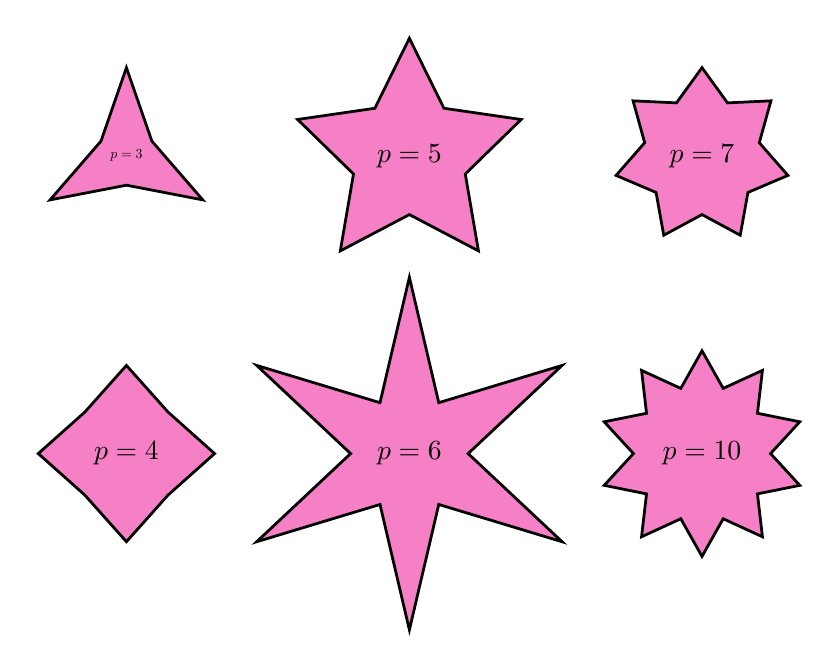
\begin{tikzpicture}[scale=2]
    \tikzstyle{ann} = [draw=none,fill=none,align=center]
    
    \matrix[nodes={draw, line width=1pt, fill=magenta!50},
        row sep=0.3cm,column sep=0.5cm] {
    \node[star,star points=3, star point ratio=3, scale=0.5] {$p=3$};&
    \node[star,star points=5,star point ratio=2] {$p=5$};&
    \node[star,star points=7] {$p=7$};
    \\
    \node[star,star points=4] {$p=4$};&
    \node[star,star points=6,star point ratio=3] {$p=6$};&
    \node[star,star points=10] {$p=10$};
    \\
    };
\end{tikzpicture}


\end{document}
